\section{Задание 1. Исследование функции одной переменной.}

\textbf{Условие.}

Изобразите данную функцию $y = f(x)$ в программах Desmos или Geogebra.

Проверьте правильность построения (если нужно уточните или скорректируйте его), проведя аналитическое исследование функции:

\begin{enumerate}
    \item $\displaystyle f(x) = 3x - \frac{2x}{|x + 2|}$
    \item $\displaystyle g(x) = \sqrt[3]{1 - |\sin{x}|}$
\end{enumerate}
\vspace{10mm}
\textbf{Решение.}


\begin{enumerate}
    \item $\displaystyle f(x) = 3x - \frac{2x}{|x + 2|} =
    \begin{sqcases}
        3x - \frac{2x}{x + 2}, x \geq -2 \\
        3x + \frac{2x}{x + 2}, x < -2
    \end{sqcases}$

    \begin{enumerate}
        \item Область определения: $D(f(x)) = \Real \setminus \Set{-2}$
        \item Разрывы, асимптоты:

        $D(f(x)) = \Real \setminus \Set{-2} \Longrightarrow -2$ - точка, в которой может быть вертикальная асимптота, проверим это:

        $\displaystyle \lim_{x \to -2^+}{f(x)} = \lim_{x \to -2^+}{3x - \frac{2x}{x + 2}} = \lim_{x \to -2^+}{\cancelto{-6}{3x} \qquad - \frac{\cancelto{-4}{2x}}{\cancelto{0^+}{x + 2}}} \quad = +\infty$

        $\displaystyle \lim_{x \to -2^-}{f(x)} = \lim_{x \to -2^-}{3x + \frac{2x}{x + 2}} = \lim_{x \to -2^-}{\cancelto{-6}{3x} \qquad + \frac{\cancelto{-4}{2x}}{\cancelto{0^-}{x + 2}}} \quad = +\infty$

        \vspace{2mm}

        $\Longrightarrow$ в точке $x = -2$ вертикальная асимптота и разрыв второго рода.

        $\displaystyle \lim_{x \to +\infty}{f(x)} = +\infty$;
        $\displaystyle \lim_{x \to +\infty}{\frac{f(x)}{x}} = 3$;
        $\displaystyle \lim_{x \to +\infty}{f(x) - 3x} = -2 \Longrightarrow $ наклонная асимптота на $+\infty$ равна $y = 3x - 2$

        $\displaystyle \lim_{x \to -\infty}{f(x)} = -\infty$;
        $\displaystyle \lim_{x \to -\infty}{\frac{f(x)}{x}} = 3$;
        $\displaystyle \lim_{x \to -\infty}{f(x) - 3x} = 2 \Longrightarrow $ наклонная асимптота на $-\infty$ равна $y = 3x + 2$

        \item Функция не является четной, нечетной и периодичной.

        \item Нули и промежутки знакопостоянства:

        $\displaystyle f(x) = 0 \Longleftrightarrow
        \begin{sqcases}
            3x - \frac{2x}{x + 2} = 0, x \geq -2 \\
            3x + \frac{2x}{x + 2} = 0, x < -2
        \end{sqcases} \Longleftrightarrow
        \begin{sqcases}
            x = 0, \\
            3 - \frac{2}{x + 2} = 0, x \geq -2 \\
            3 + \frac{2}{x + 2} = 0, x < -2
        \end{sqcases} \Longleftrightarrow
        \begin{sqcases}
            x = 0, \\
            \frac{1}{x + 2} = \frac{3}{2}, x \geq -2 \\
            \frac{1}{x + 2} = -\frac{3}{2}, x < -2
        \end{sqcases} \Longleftrightarrow
        \begin{sqcases}
            x = 0, \\
            x = \frac{2}{3} - 2 = -\frac{4}{3}, x \geq -2 \\
            x = - \frac{2}{3} - 2 = -\frac{8}{3}, x < -2
        \end{sqcases}$

        На интервалах $\displaystyle \left(-\infty; -\frac{8}{3}\right) \union \left(-\frac{4}{3}; 0\right)$ $f(x) < 0$,

        на интервалах $\displaystyle \left(-\frac{8}{3}; -2\right) \union \left(2; -\frac{4}{3}\right) \union (0; +\infty)$ $f(x) > 0$

        \item Экстремумы:

        $f^\prime(x) =
        \begin{sqcases}
            \left(3x - \frac{2x}{x + 2}\right)^\prime, x \geq -2 \\
            \left(3x + \frac{2x}{x + 2}\right)^\prime, x < -2
        \end{sqcases} =
        \begin{sqcases}
            3 - \frac{2(x + 2) - 2x}{(x + 2)^2}, x \geq -2 \\
            3 + \frac{2(x + 2) - 2x}{(x + 2)^2}, x < -2
        \end{sqcases} =
        \begin{sqcases}
            3 - \frac{4}{(x + 2)^2}, x \geq -2 \\
            3 + \frac{4}{(x + 2)^2}, x < -2
        \end{sqcases}$

        $f^\prime(x) = 0 \Longleftrightarrow
        \begin{sqcases}
            3 - \frac{4}{(x + 2)^2} = 0, x \geq -2 \\
            3 + \frac{4}{(x + 2)^2} = 0, x < -2
        \end{sqcases} \Longleftrightarrow
        \begin{sqcases}
        (x + 2)
            ^2 = \frac{4}{3}, x \geq -2\\
            x \notin \Real
        \end{sqcases} \Longleftrightarrow x = -2 + \frac{2\sqrt{3}}{3}$ - экстремум

        При $x > -2 + \frac{2\sqrt{3}}{3}$ $f^\prime(x) > 0$, $x < -2 + \frac{2\sqrt{3}}{3}$ $f^\prime(x) < 0$ $\Longrightarrow$
        в точке $x = -2 + \frac{2\sqrt{3}}{3}$ минимум функции

        \item Перегибы и выпуклости:

        $f^{\prime\prime}(x) =
        \begin{sqcases}
            \left(3 - \frac{4}{(x + 2)^2})^\prime, x \geq -2 \\
            \left(3 + \frac{4}{(x + 2)^2})^\prime, x < -2
        \end{sqcases} =
        \begin{sqcases}
            \left(3 - 4(x + 2)^{-2})^\prime, x \geq -2 \\
            \left(3 + 4(x + 2)^{-2})^\prime, x < -2
        \end{sqcases} = \\
        = \begin{sqcases}
              8(x + 2)^{-3} > 0, x \geq -2 \text{ - функция выпукла вниз} \\
              -8(x + 2)^{-3} > 0, x < -2 \text{ - функция выпукла вниз}
        \end{sqcases}$

        Точек перегибов нет.

        \item График (источник - \url{https://www.desmos.com/calculator/oaz4rrr735}):

        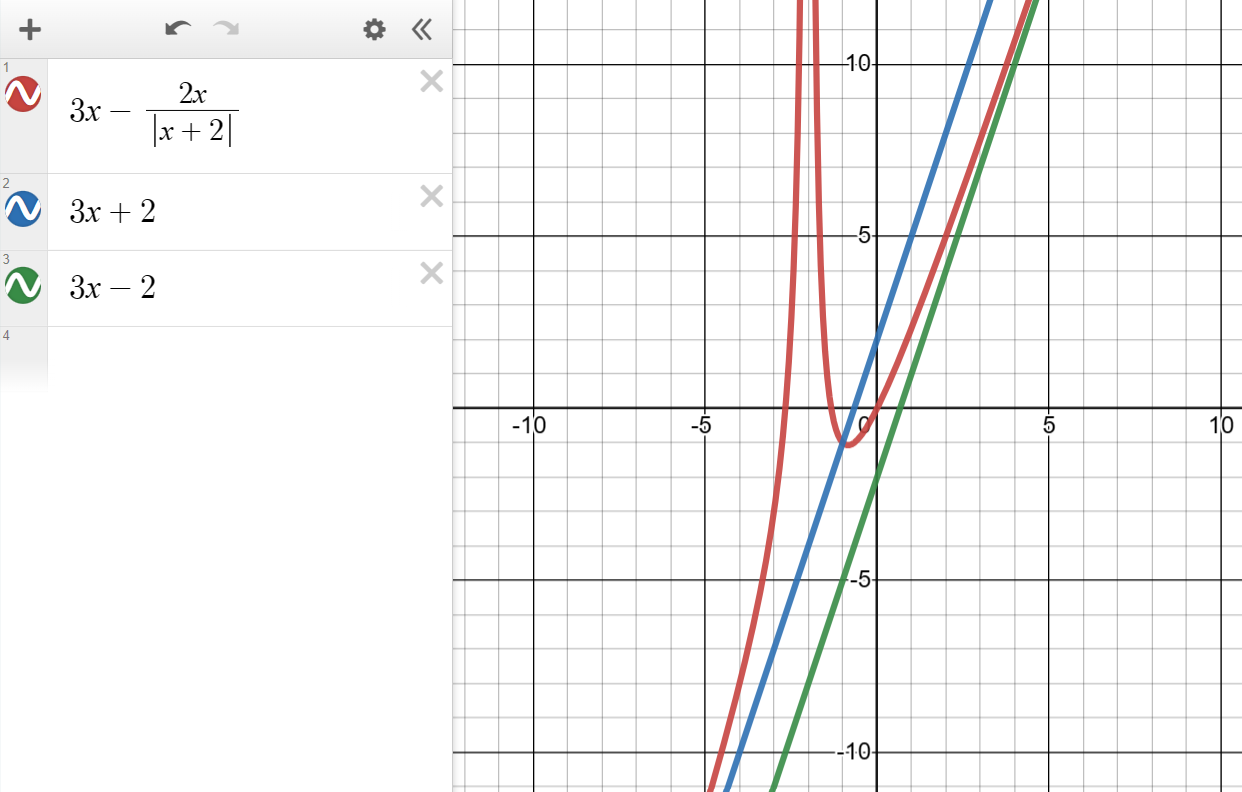
\includegraphics[width=14cm]{images/1a1}

    \end{enumerate}



    \item $\displaystyle g(x) = \sqrt[3]{1 - |\sin{x}|}$

    \begin{enumerate}
        \item Область определения:

        $D(g(x)) = \Real$; \quad
        $E(g(x)) = [0; 1]$

        \item Разрывы, асимптоты:

        $D(g(x)) = \Real \Longrightarrow$ - вертикальных асимптот нет

        $\displaystyle g(x) = \sqrt[3]{1 - |\sin{x}|} =
        \begin{sqcases}
            \sqrt[3]{1 - \sin{x}}, \quad \sin{x} \geq 0 \quad (2\pi k \leq x \leq 2\pi k + \pi, k \in \Integer) \\
            \sqrt[3]{1 + \sin{x}} = \sqrt[3]{1 - \sin{x + \pi}}, \quad \sin{x} < 0 \quad (2\pi k + \pi < x < 2\pi (k + 1), k \in \Integer)
        \end{sqcases}$

        Функция имеет период $\pi$, поэтому $\displaystyle \nexists \lim_{x \to\infty}{g(x)}$, поэтому наклонных асимптот нет

        \item Функция имеет период $\pi$

        \item Нули и промежутки знакопостоянства:

        $g(x) = 0 \Longleftrightarrow \sqrt[3]{1 - |\sin{x}|} = 0 \Longleftrightarrow \\
        1 - |\sin{x}| = 0 \Longleftrightarrow \sin{x} = \pm 1 \Longleftrightarrow x = \frac{\pi}{2} + \pi k (k \in \Integer)$

        Так как $E(g(x)) = [0; 1]$ функция всегда не отрицательна.
        \item Экстремумы:

        $g^\prime(x) =
        \begin{sqcases}
            \left((1 - \sin{x})^{1/3}\right)^\prime, \quad \sin{x} \geq 0 \\
            \left((1 - \sin(x + \pi))^{1/3}\right)^\prime, \quad \sin{x} < 0
        \end{sqcases} =
        \begin{sqcases}
            -\frac{\cos{x}}{3}(1 - \sin{x})^{-2/3}, \quad \sin{x} \geq 0 \\
            -\frac{\cos{(x + \pi)}}{3}(1 - \sin(x + \pi))^{-2/3}, \quad \sin{x} < 0
        \end{sqcases}$

        $1 \pm \sin{x} \neq 0 \Longrightarrow \sin{x} \neq \pm 1 \Longrightarrow x \neq \frac{\pi}{2} + \pi k \quad (k \in \Integer)$

        $g(x) = 0 \Longleftrightarrow
        \begin{sqcases}
            \cos{x} = 0, \text{ - производная не существует} \\
            \sin{x} = \pm 1 \text{ - производная не существует}
        \end{sqcases} \Longleftrightarrow $ в точках $x = \frac{\pi}{2} + \pi k (k \in \Integer)$ экстремумы


        \item Перегибы и выпуклости:

        $g^{\prime\prime}(x) =
        \begin{sqcases}
            \left(-\frac{\cos{x}}{3}(1 - \sin{x})^{-2/3}\right)^\prime, \quad \sin{x} \geq 0 \\
            \left(-\frac{\cos{(x + \pi)}}{3}(1 - \sin(x + \pi))^{-2/3}\right)^\prime, \quad \sin{x} < 0
        \end{sqcases} = \\
        \begin{sqcases}
            \frac{\sin{x}}{3}(1 - \sin{x})^{-2/3} + \frac{-2\cos{x}\cos{x}}{9}(1 - \sin{x})^{-5/3}, \quad \sin{x} \geq 0 \\
            \frac{\sin(x + \pi)}{3}(1 - \sin(x + \pi))^{-2/3} + \frac{-2\cos(x + \pi)\cos(x + \pi)}{9}(1 - \sin(x + \pi))^{-5/3}, \quad \sin{x} < 0
        \end{sqcases} = \\
        \begin{sqcases}
            (1 - \sin{x})^{-2/3}\left(\frac{3\sin{x} - 3\sin^2{x} - 2\cos^2{x}}{9 (1 - \sin{x})}\right), \quad \sin{x} \geq 0 \\
            (1 - \sin(x + \pi))^{-2/3}\left(\frac{3\sin(x + \pi) - 3\sin^2(x + \pi) - 2\cos^2(x + \pi)}{9 (1 - \sin(x + \pi))}\right), \quad \sin{x} < 0 \\
        \end{sqcases} = \\
        \begin{sqcases}
            -(1 - \sin{x})^{-2/3}\left(\frac{(\sin{x} - 1)(\sin{x} - 2)}{9 (1 - \sin{x})}\right), \quad \sin{x} \geq 0 \\
            -(1 - \sin(x + \pi))^{-2/3}\left(\frac{(\sin(x + \pi) - 1)(\sin(x + \pi) - 2)}{9 (1 - \sin(x + \pi))}\right), \quad \sin{x} < 0 \\
        \end{sqcases}$

        $(\sin{x} - 1)(\sin{x} - 2) > 0$ при $\sin{x} \geq 0$, $(1 - \sin{x}) \in (0;1]$ при $\sin{x} \geq 0$ (аналогично для второй части уравнения)
        $\Longrightarrow g^{\prime\prime}(x) < 0$ на всем промежутке, а функция выпукла вверх

        \item График (источник - \url{https://www.desmos.com/calculator/m342woai2d}):

        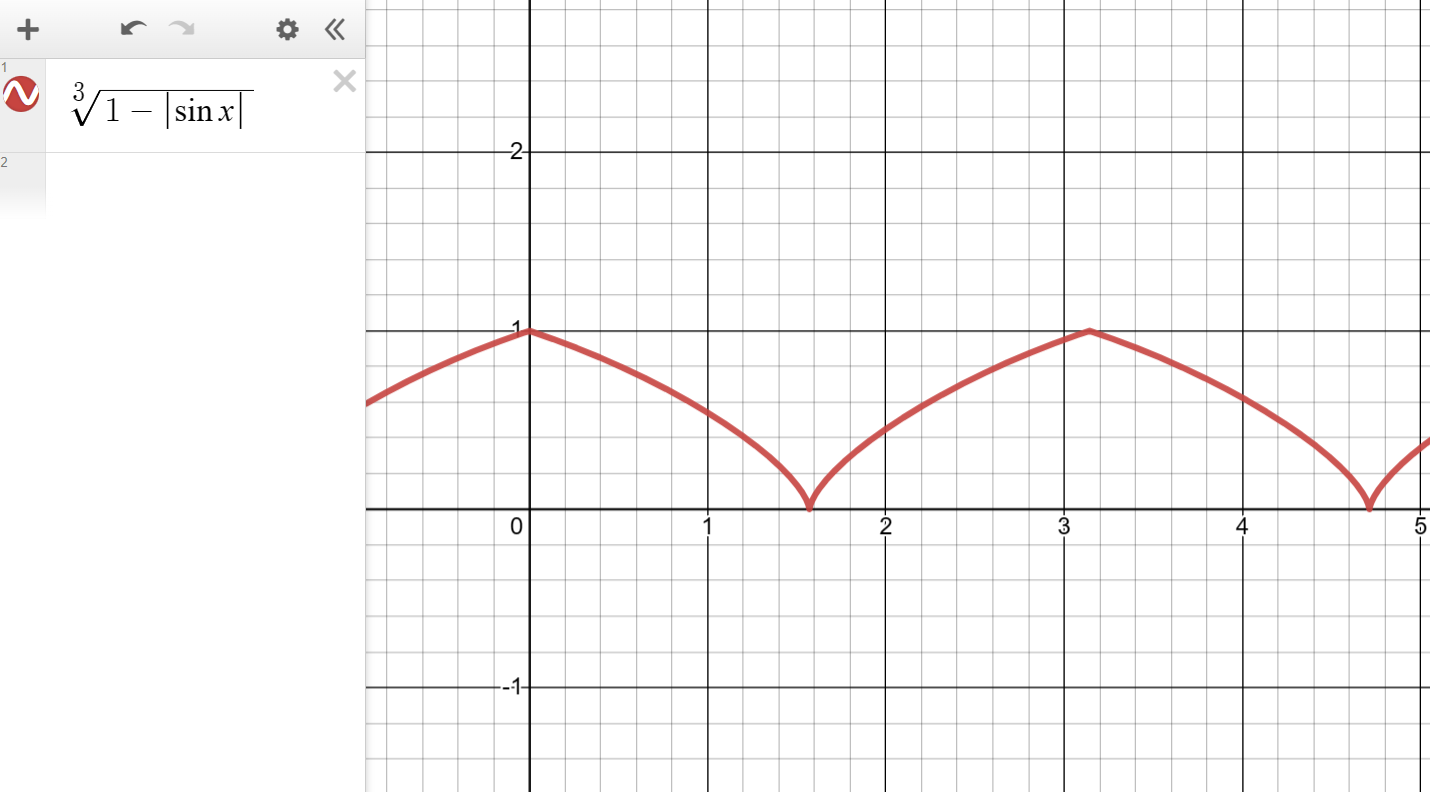
\includegraphics[width=14cm]{images/1b1}

    \end{enumerate}
\end{enumerate}

\clearpage
